\documentclass[11pt]{amsart}
\usepackage{geometry}                % See geometry.pdf to learn the                                                                                                                                                                                                                      
                                % layout options. There are lots.                                                                                                                                                                                                                         
\geometry{letterpaper}                   % ... or a4paper or a5paper                                                                                                                                                                                                                      
                                % or ...                                                                                                                                                                                                                                                  
%\geometry{landscape}                % Activate for for rotated page                                                                                                                                                                                                                      
%geometry                                                                                                                                                                                                                                                                                 
%\usepackage[parfill]{parskip}    % Activate to begin paragraphs with                                                                                                                                                                                                                     
%an empty line rather than an indent                                                                                                                                                                                                                                                      
\usepackage{graphicx}
\usepackage{amssymb}
\usepackage{epstopdf}
\DeclareGraphicsRule{.tif}{png}{.png}{`convert #1 `dirname
  #1`/`basename #1 .tif`.png}
\usepackage{hyperref}
\usepackage{/Library/Frameworks/R.framework/Resources/share/texmf/Sweave}

\title{Foundation species genetics structures lichen community
  interaction networks}
\author{M.K. Lau, L.J. Lamit, T.G. Whitham}
%\date{}                                           % Activate to                                                                                                                                                                                                                          
%display a given date or no date                                                                                                                                                                                                                                                          

\begin{document}
\maketitle


\setcounter{tocdepth}{1}
\tableofcontents


%%%chunk0

%%%chunk1


%%%chunk2


%%%chunk3

%%%chunk4


%%%chunk5


%%%chunk6

%%%chunk7



%%%chunk8


%%%chunk9



%%%chunk10

%%%Figure for macrobiology grant


%%%chunk11


%%%chunk11

%%%chunk12

\textbf{Take-Home:} Foundation species genetics influences the structure of
  interactions among bark lichen species most likely by altering the
  trajectory of community assembly.

\section{Abstract}
\begin{itemize}
\item Understanding the complexities of community dynamics requires a
  greater understanding of the interactions among species and the
  forces that influence the structure of these interactions. 
\item We present a study of bark lichen communities associated with
  \textit{Populus angustifolia} (narrowleaf cottonwood), where we
  applied quantitative network modeling to investigate the genetic
  effects of a foundation tree species on bark-lichen community
  interactions networks.
\item There were three main findings:
  \begin{enumerate}
  \item Genotype significantly predicted the similarity of lichen
    interactions networks. Species richness explained additional
    variation in network similarity.
  \item Both genotype and richness significantly predicted the
    variation in three network structural metrics (size, degree and
    centralization). 
  \item All network metrics were highly correlated with each other and
    lichen species richness. Thus, after controlling for the variation explained by lichen
    species richness, all three network metrics significantly
    predicted variation in the similarity of networks but only
    network size explained a biologically relevant amount of variation
    in network similarity. 
  \end{enumerate}
\item These results strongly support the hypothesis that there is a
  genetic component to the structure of species interactions. Our
  quantative network modeling and network analyses show that this
  genetic effect is not due to variation in lichen species richness
  arising from genotype, but by some other causal pathway. These
  results indicate that the variation in network structure among
  genotypes arises from the communities being at different levels of
  community assembly, as both species richness and the size of the
  network independently explained the most variation in network similarity.
\item These findings are particularly important as they suggest that
  quantitative modeling of community-wide interaction networks can aid
  our understanding of community dynamics and that we need to place
  interactions among species within an evolutionary framework.
\end{itemize}

\section{Introduction}
\begin{itemize}
\item Understanding complex species interactions is important for
  ecology (reviewed in Bascompte 2009, and others...). 
\item A substantial body of evidence provides support for the value in
  putting communities and ecosystems into an evolutionary framework
  (reviewed in PRS-B 2011, Johnson and Agrawal 200?, Whitham et
  al. 2008 and Whitham et al. 2007). However, there is still little
  known about how genetic variation in a foundation species affects
  the interactions among multiple species in complex communities (but
  see Bailey et al 2005).
\item Defining species interactions and obtaining quantitative data
  for interactions in complex communities presents a challenge to
  ecologists.
\item Newly developed quantitative network modeling methods provide
  one means to not only obtain estimates of species interactions but
  also circumvent the need to limit interactions to one or few
  categories (e.g. trophic, mutualistic or host-parasite
  interactions).
\item Here, we present the results of a study of how foundation
  species genetics influences variation in interactions among multiple
  species.
\end{itemize}

\section{Methods}
\begin{itemize}
\item Garden description. 
\item Samling description. The presence of bark lichen species were
  assessed within 50 replicate 1 cm$^2$ grid cells of 10 cm$^2$
  quadrats on replicate clones of known genotype in a  common garden
  at the Ogden Nature Center (Utah, USA). 50 out of the  100 cells in
  each quadrat were sampled in a checker-board pattern in  order to
  minimize the probability of individuals overlapping between
  cells. 122 trees sampled, 13 genotypes, 5800 grid cells.
\item Network modeling. Network models were generated using a
  correlation based algorithm to detect species interactions on each
  individual tree. Thus, we produced a quantitative, undirected model
  of species interactions on each individual tree.
\item Statistical methods for network similarity. We then applied
  network analyses and mutlivariate statistical methods to test for
  the effect of genotype on lichen community interaction network
  structure. In order to compare networks, we measured the similarity
  between networks as the sum of the Euclidean distance for all edges
  between each network pair for all networks. This formed a distance
  matrix that we then used in PerMANOVA analyses of the factors
  influencing network similarity. We used ANOVA to analyze the effect
  of genotype and richness on the network structural metrics. To
  visualize the similarity of network genotypes, we applied prinicipal
  components analysis to the network distances and used ordination
  vector fitting methods to explore the possible sources of similarity
  among netowrks. 
\end{itemize}

\section{Results}

\begin{enumerate}
\item We found significant variation in network structure among tree
  genotypes (Fig. 1). Genotype and lichen species richness were both
  significant predictors of the structural similarity of the lichen community networks with genotype
  and richness explaining
  29\% and
  17\% of the
  variation in lichen network similarity (Table 1). 
\item We investigated several network statistics to explore the
  structural variation responsible for the variation in network
  similarity and found that genotype and richness significantly
  predicted the variation in all three network metrics (Fig. 2 and
  Tables 2-4). Note that bark roughness was not a significant
  predictor of network similarity ($p = $ 0.489).
\item  All network metrics were highly correlated with each other and
  lichen species richness (Fig. 3). Thus, after controlling for the variation explained by lichen
  species richness, all three network metrics significantly
  predicted variation in the similarity of networks but only
  network size explained a biologically relevant amount of variation
  in network similarity.  ($r^2 = $
  0.02) after
  controlling for the variation explained by lichen species richness
  (Table 5).
\end{enumerate}


\section{Conclusion}

\begin{itemize}
\item Genotype influences the size, degree and centralization of
  lichen community interaction networks. It is important to note
  that none of these network metrics were significantly predicted by
  the number of trees sampled for a given genotype (i.e. variation in
  the number of observations did not produce these patterns). 
\item This pattern does not seem to be related to the bark roughness,
  as richness and community composition seem to be. This is
  intriguing since roughness seems to be an important
  factor in lichen establishment and a good predictor of the genotype
  effect on the distribution of the dominant lichen species (Lamit et
  al. 2010).
\item These results are particularly striking given that lichen
  species are very slow growing and that our communities are all
  likely to be in the early stages of establishment.
\item These findings are important as they present a
  step toward putting complex, community-wide
  interactions in an evolutionary framework.
\end{itemize}


\pagebreak

%Table 1. PerMANOVA table for genotype x richness model
%%%chunk13
\begin{center} 
% latex table generated in R 2.14.0 by xtable 1.6-0 package
% Wed Mar  7 12:31:39 2012
\begin{table}[ht]
\begin{center}
\begin{tabular}{lrrrrrr}
  \hline
 & Df & SumsOfSqs & MeanSqs & F.Model & R2 & Pr($>$F) \\ 
  \hline
Genotype & 13 & 0.94 & 0.07 & 2.54 & 0.29 & 0.0071 \\ 
  Richness & 1 & 0.55 & 0.55 & 19.48 & 0.17 & 0.0001 \\ 
  Genotype:Richness & 12 & 0.81 & 0.07 & 2.38 & 0.25 & 0.0054 \\ 
  Residuals & 34 & 0.97 & 0.03 &  & 0.30 &  \\ 
  Total & 60 & 3.27 &  &  & 1.00 &  \\ 
   \hline
\end{tabular}
\caption{ANOVA table for the PerMANOVA test of the effect of genotype and lichen species richness on the similarity of the lichen interaction networks.}
\end{center}
\end{table}\end{center} 

\pagebreak

%Table 2-4. ANOVA tables for the effect of genotype and richness on the
%structural statistics.
%%%chunk14
\begin{center} 
% latex table generated in R 2.14.0 by xtable 1.6-0 package
% Wed Mar  7 12:31:39 2012
\begin{table}[ht]
\begin{center}
\begin{tabular}{lrrrrr}
  \hline
 & Df & Sum Sq & Mean Sq & F value & Pr($>$F) \\ 
  \hline
Genotype          & 13 & 43.48 & 3.34 & 3.21 & 0.0032 \\ 
  Richness          & 1 & 37.32 & 37.32 & 35.80 & 0.0000 \\ 
  Genotype:Richness & 12 & 7.94 & 0.66 & 0.63 & 0.7976 \\ 
  Residuals         & 34 & 35.45 & 1.04 &  &  \\ 
   \hline
\end{tabular}
\caption{ANOVA table for the tests of the effects of genotype and richness on network size (i.e. the number of species in the network).}
\end{center}
\end{table}\end{center} 

%%%chunk15
\begin{center} 
% latex table generated in R 2.14.0 by xtable 1.6-0 package
% Wed Mar  7 12:31:39 2012
\begin{table}[ht]
\begin{center}
\begin{tabular}{lrrrrr}
  \hline
 & Df & Sum Sq & Mean Sq & F value & Pr($>$F) \\ 
  \hline
Genotype          & 13 & 10.99 & 0.85 & 2.97 & 0.0054 \\ 
  Richness          & 1 & 8.89 & 8.89 & 31.21 & 0.0000 \\ 
  Genotype:Richness & 12 & 1.80 & 0.15 & 0.53 & 0.8819 \\ 
  Residuals         & 34 & 9.68 & 0.28 &  &  \\ 
   \hline
\end{tabular}
\caption{ANOVA table for the tests of the effects of genotype and richness on network degree (i.e. the number of connections).}
\end{center}
\end{table}\end{center} 

%%%chunk16
\begin{center} 
% latex table generated in R 2.14.0 by xtable 1.6-0 package
% Wed Mar  7 12:31:39 2012
\begin{table}[ht]
\begin{center}
\begin{tabular}{lrrrrr}
  \hline
 & Df & Sum Sq & Mean Sq & F value & Pr($>$F) \\ 
  \hline
Genotype          & 13 & 0.48 & 0.04 & 2.35 & 0.0229 \\ 
  Richness          & 1 & 0.36 & 0.36 & 22.74 & 0.0000 \\ 
  Genotype:Richness & 12 & 0.06 & 0.00 & 0.29 & 0.9865 \\ 
  Residuals         & 34 & 0.54 & 0.02 &  &  \\ 
   \hline
\end{tabular}
\caption{ANOVA table for the tests of the effects of genotype and richness on network centralization (i.e. the degree to which the network is dominated by one species).}
\end{center}
\end{table}\end{center} 

\pagebreak

%Table 3. PerMANOVA of the effect of the three metrics after removing
%the variance explained by richness.
%%%chunk17
\begin{center} 
% latex table generated in R 2.14.0 by xtable 1.6-0 package
% Wed Mar  7 12:31:39 2012
\begin{table}[ht]
\begin{center}
\begin{tabular}{lrrrrrr}
  \hline
 & Df & SumsOfSqs & MeanSqs & F.Model & R2 & Pr($>$F) \\ 
  \hline
Richness & 1 & 0.85 & 0.85 & 21.20 & 0.26 & 0.0001 \\ 
  Size & 1 & 0.05 & 0.05 & 1.32 & 0.02 & 0.2537 \\ 
  Degree & 1 & 0.04 & 0.04 & 1.04 & 0.01 & 0.3306 \\ 
  Centralization & 1 & 0.08 & 0.08 & 2.09 & 0.03 & 0.1463 \\ 
  Residuals & 56 & 2.24 & 0.04 &  & 0.69 &  \\ 
  Total & 60 & 3.27 &  &  & 1.00 &  \\ 
   \hline
\end{tabular}
\caption{ANOVA table for the PerMANOVA test of the effects of the network metrics (size, degree and centralization) on network similarity after removing the variance explained by richness.}
\end{center}
\end{table}\end{center} 

\pagebreak

%Figure 1 is the mean network graphs for each genotype.
%%%chunk18
\begin{figure} 
\begin{center} 
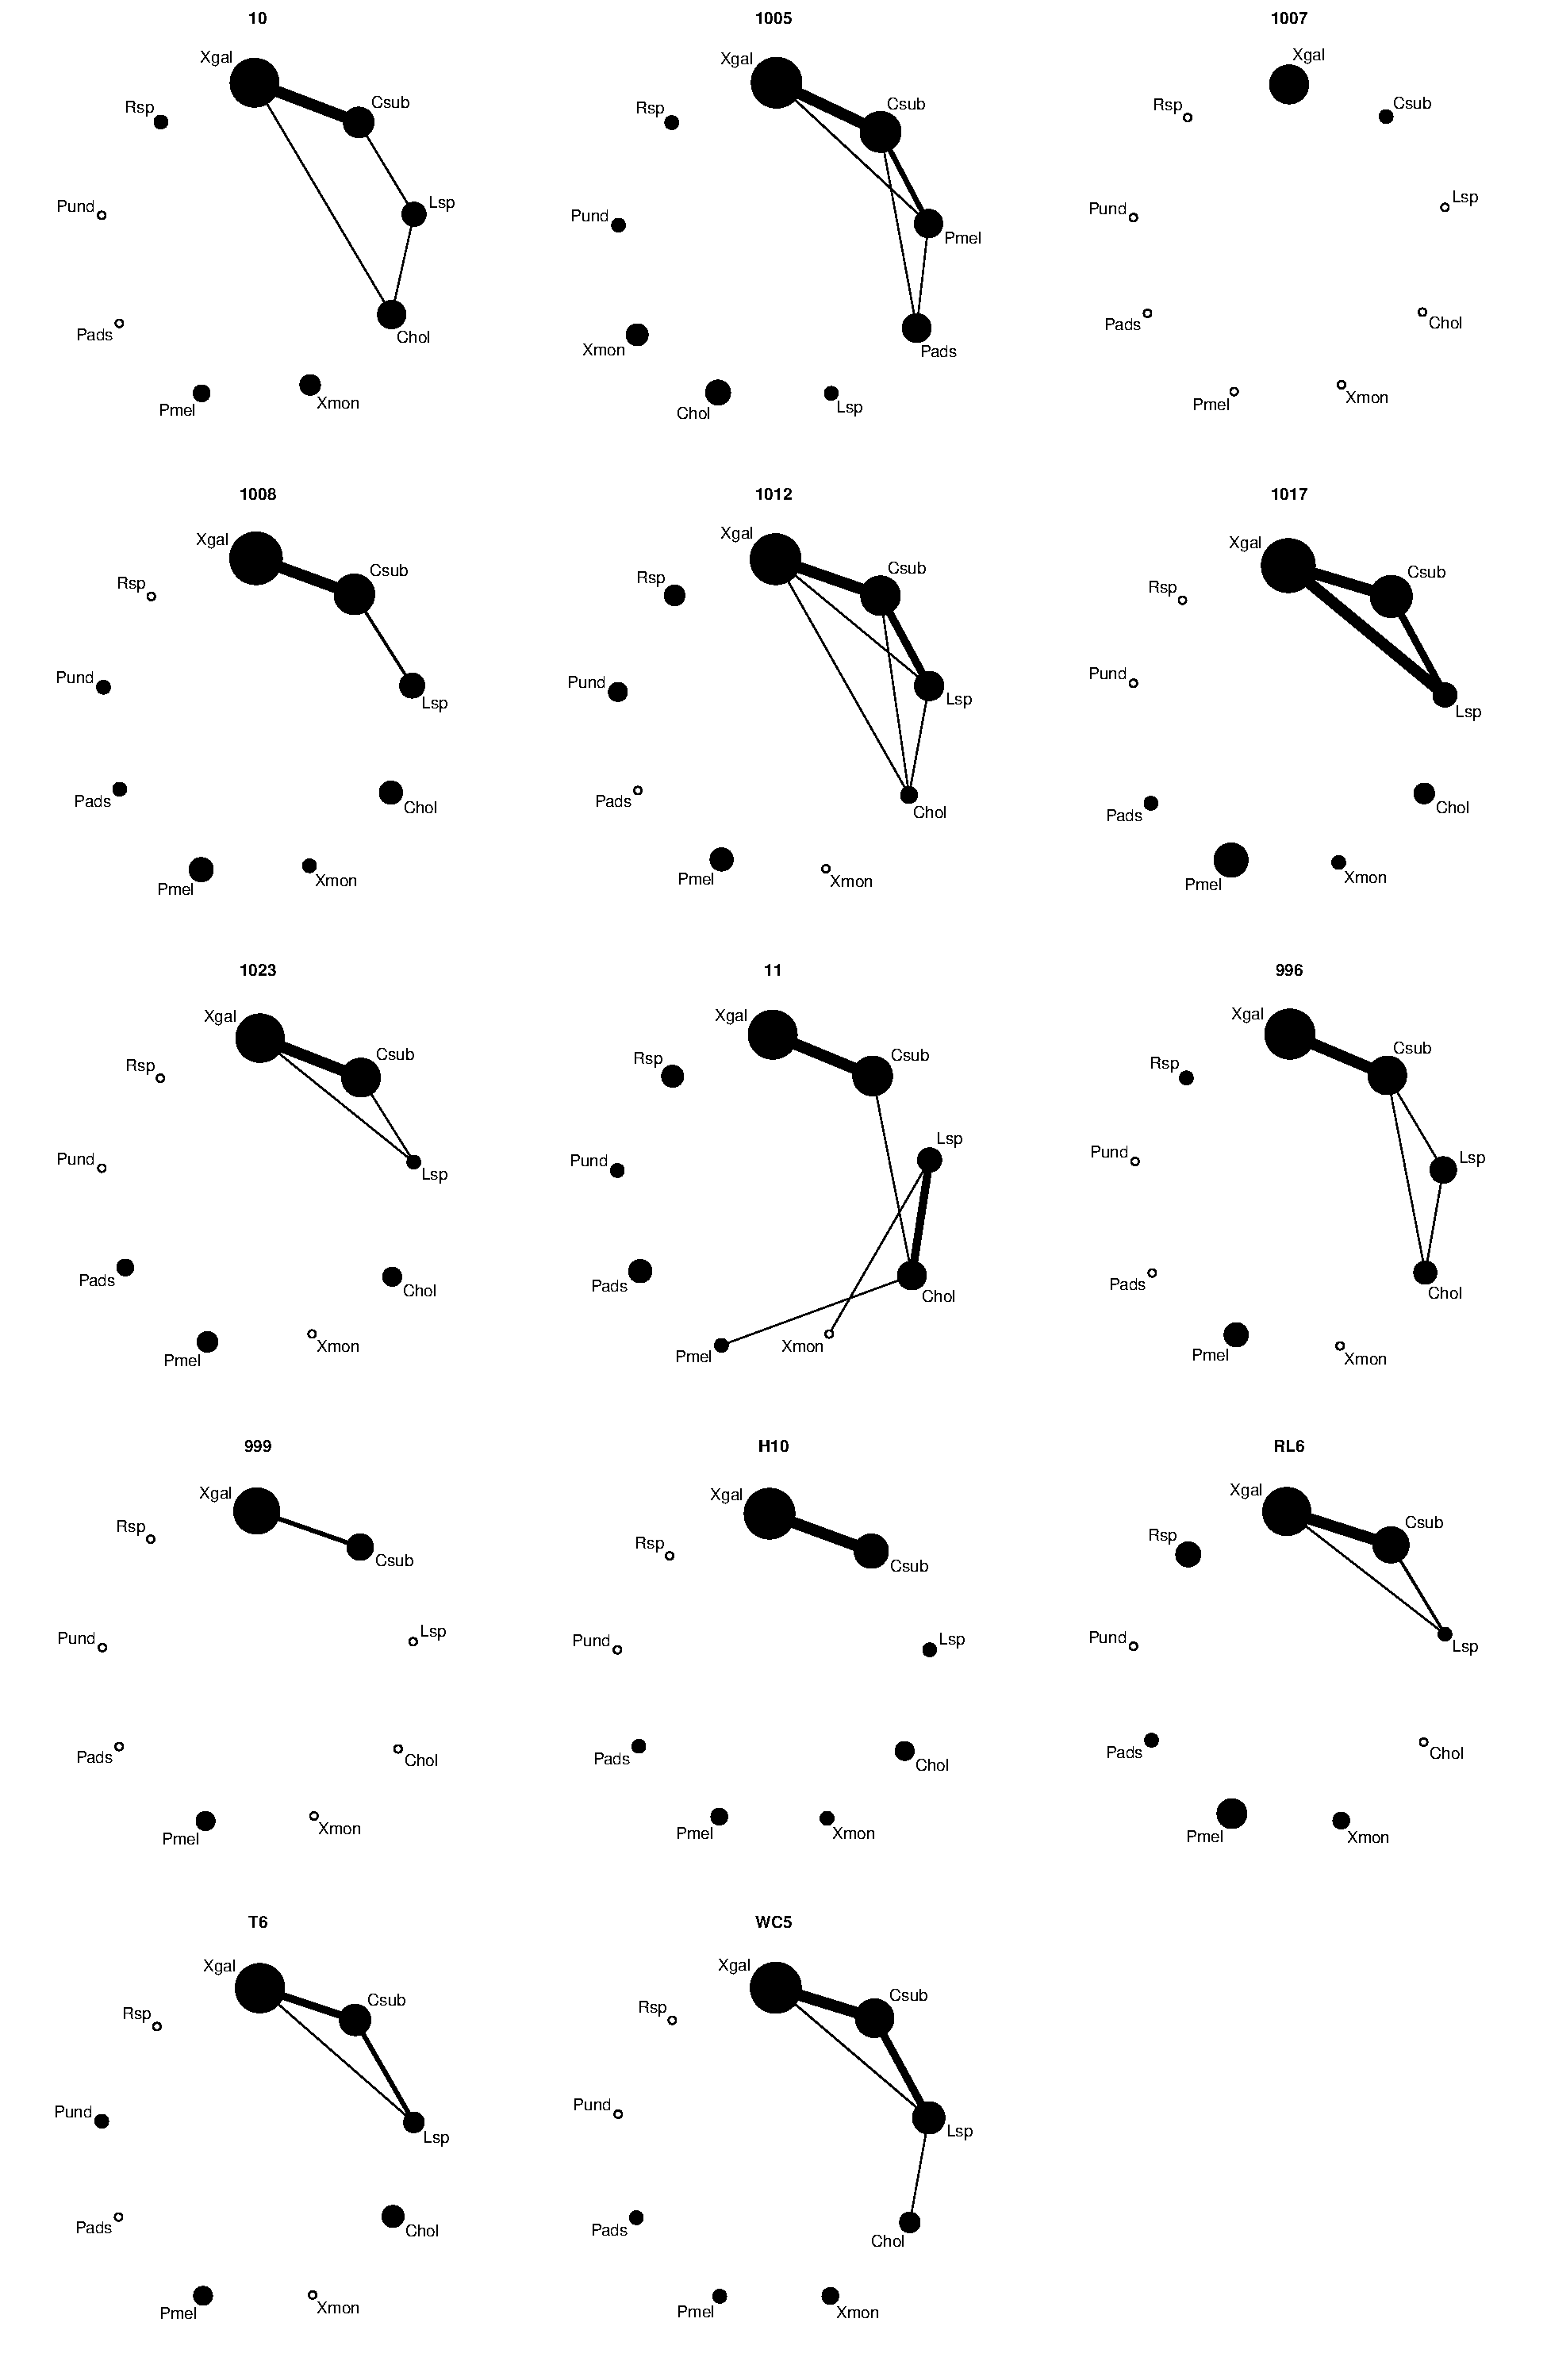
\includegraphics{ONC_Lichen_Summary-gplots}
\end{center} 
\caption{Network graphs for each genotype. Points represent species scaled by
the log of there total frequency of occurrence and lines show the
means of significant connections between species across genotype
replicates scaled by their magnitudes. Species points that had zero
frequencies are colored white.}

\label{fig:one}
\end{figure}


%Figure 2 is the ordination plot with the vectors.
%%%chunk19

\begin{figure} 
\begin{center} 
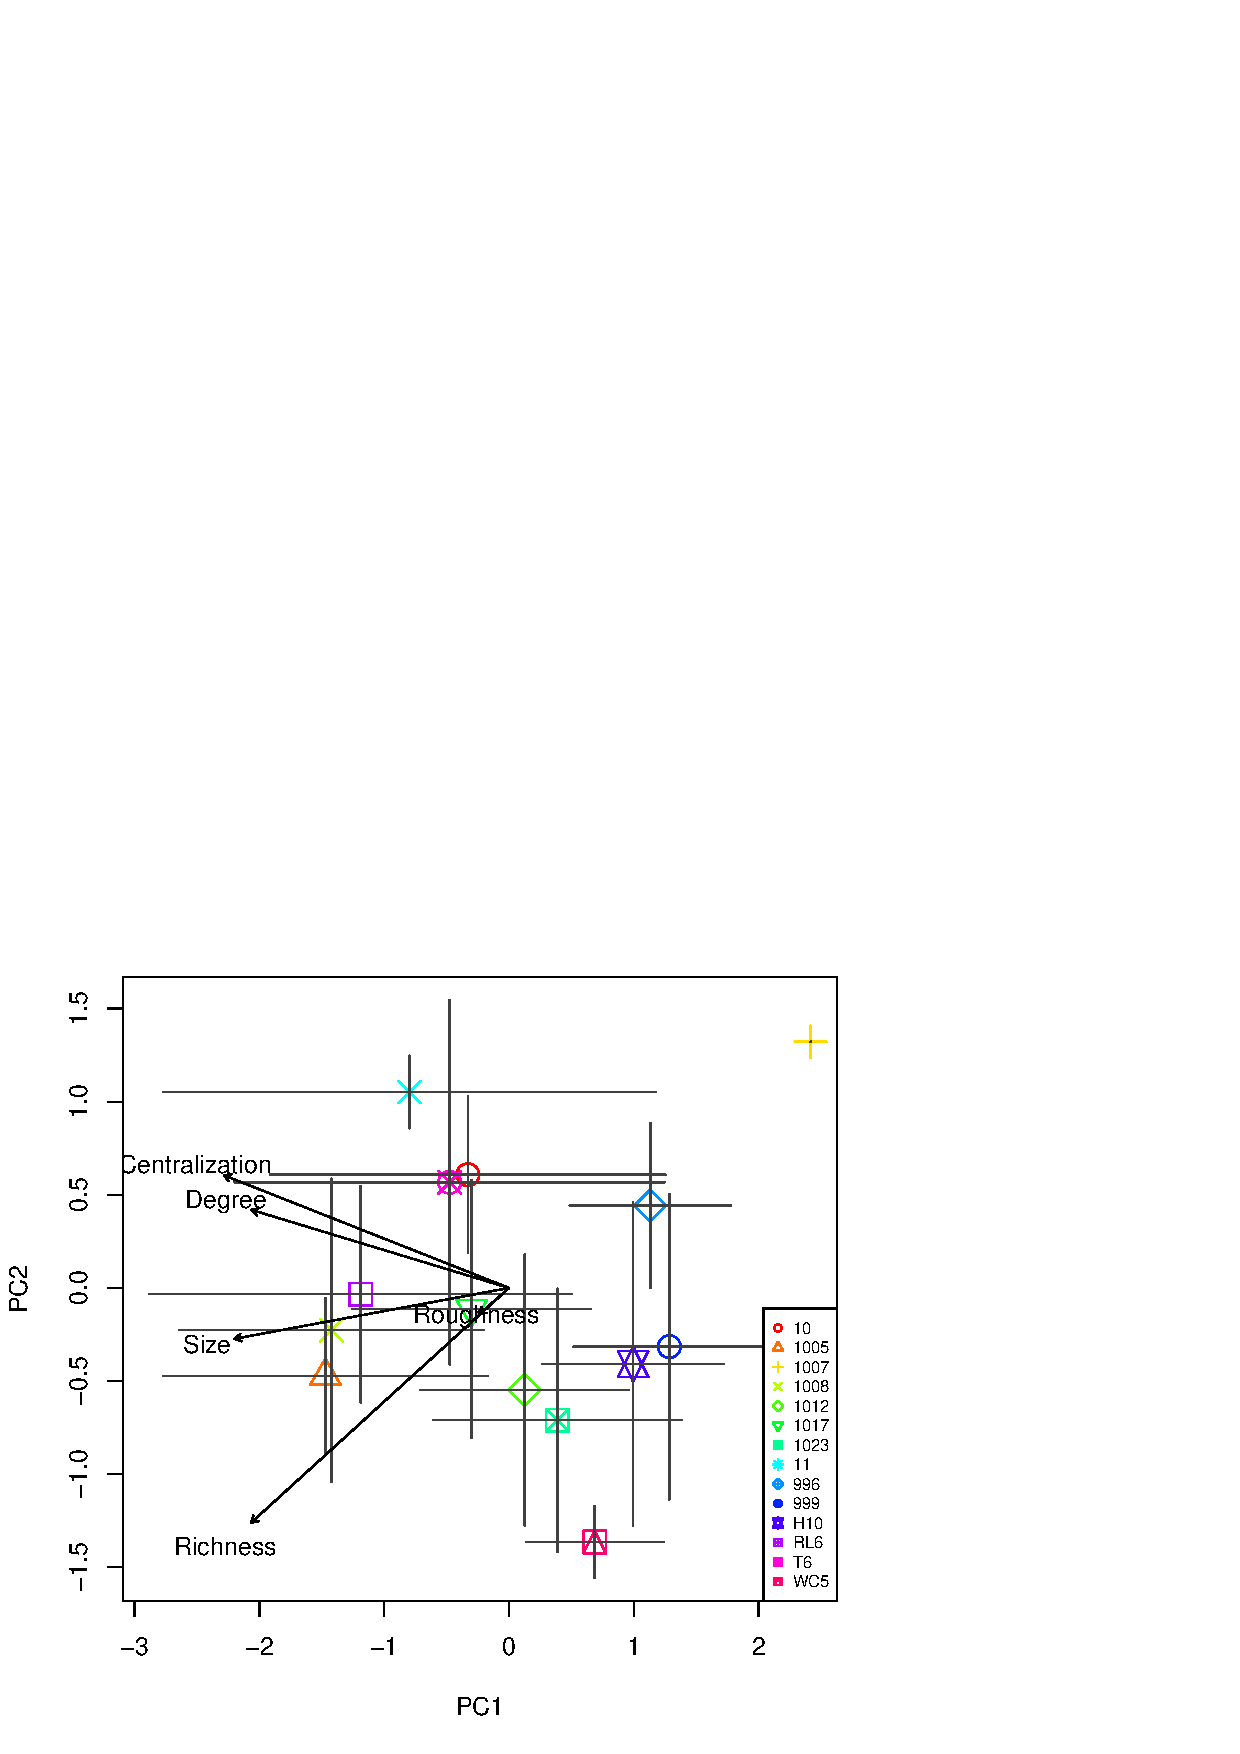
\includegraphics{ONC_Lichen_Summary-ordinet}
\end{center} 
\caption{Principle components ordination plot of the similarity
  between networks. Points represent the genotype means for the
  ordinated scores and bars show the spread (1 S.E.). Vectors show the
strength (vector length) and the direction of spread networks (vector
direction) of the correlation between roughness, the network metrics
(size, degree and centralization) and richness and the ordinated
networks.}
\label{fig:two}
\end{figure}


%Figure 3 is the pairs plot of the relationship between richness and
%the three network structural variables.
%%%chunk20
\begin{figure} 
\begin{center} 
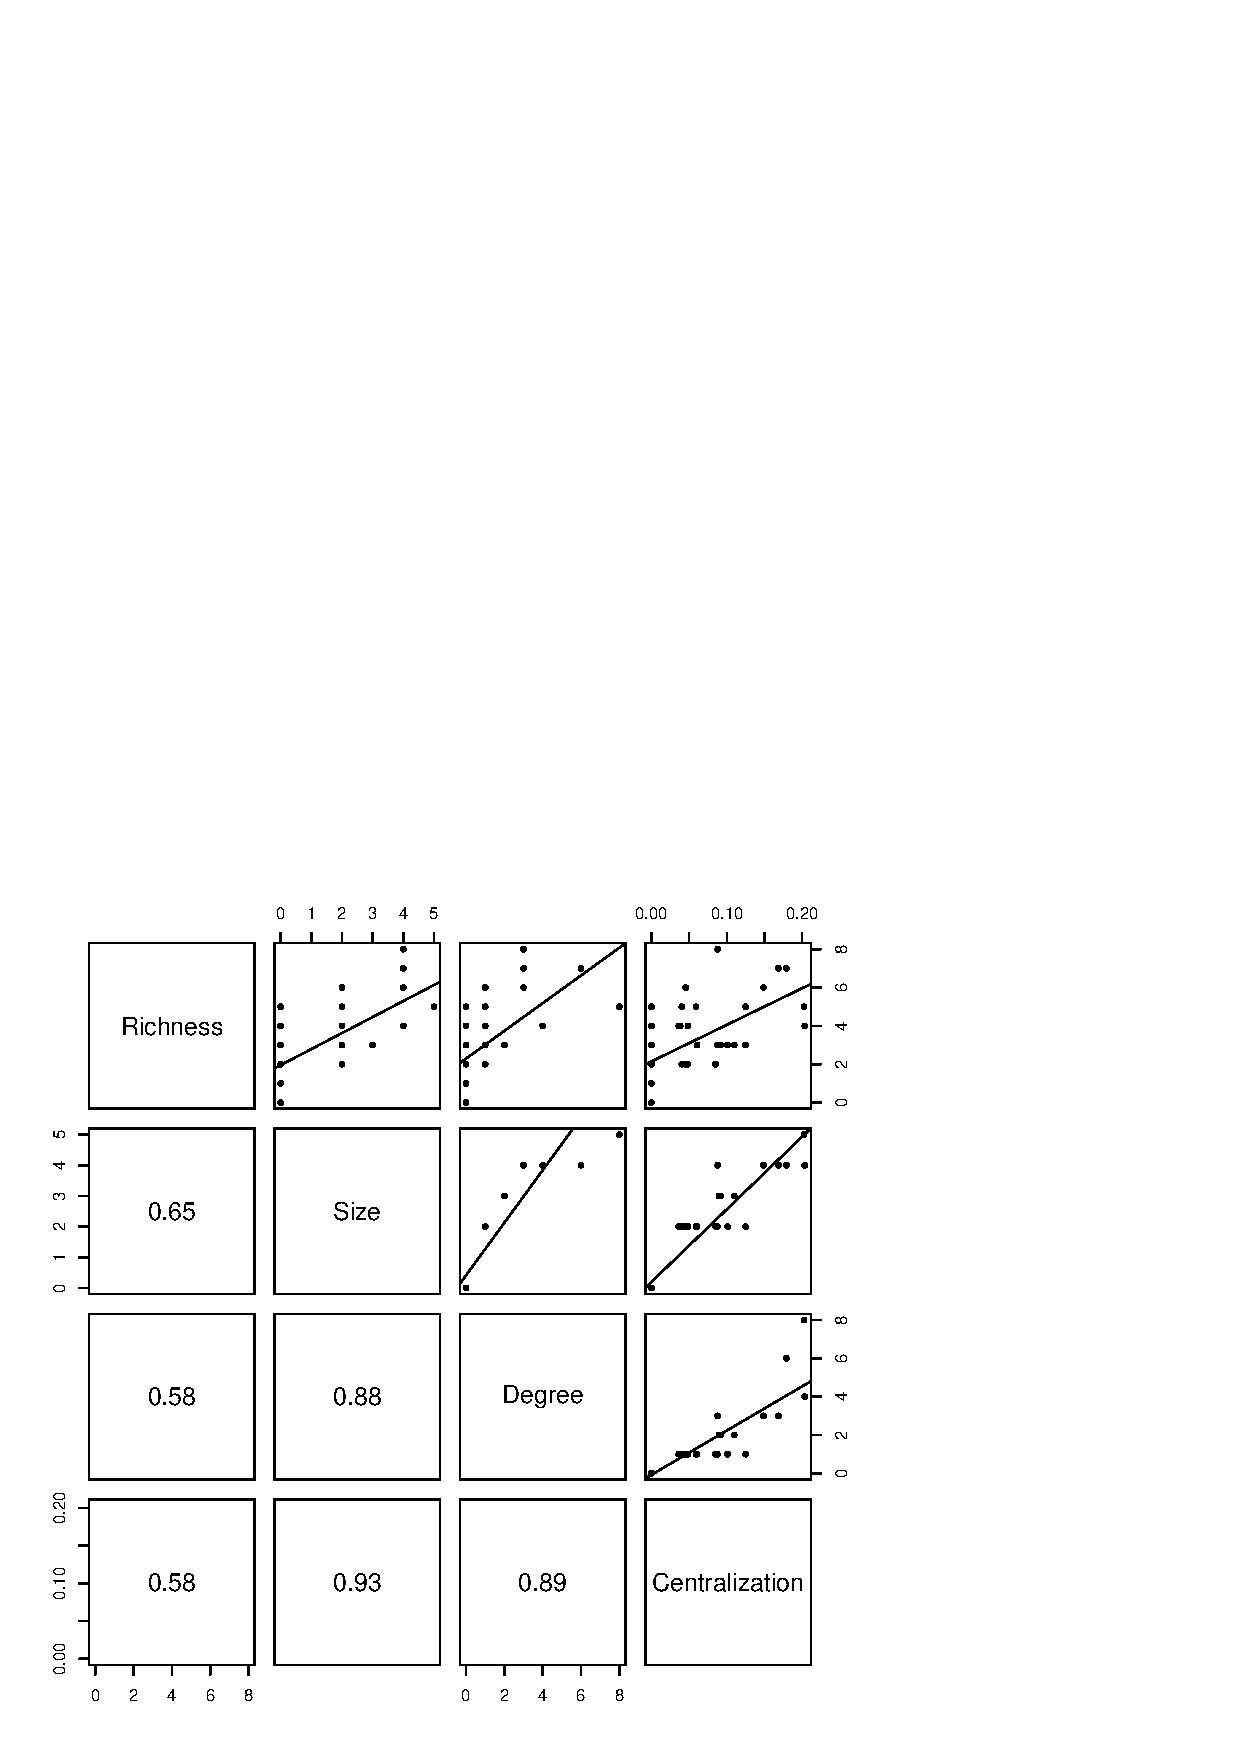
\includegraphics{ONC_Lichen_Summary-pairsplot}
\end{center} 
\caption{Matrix of bivariate plots for the network structure
  statistics (size = number of species in the network, degree = number
of connections and centralization = dominance of the network by one
species) and species richness (measured as the number of species
present in the quadrat). Note that although a species may have been
present in a quadrat, it may not have a significant connection to
any other species in the community.}
\label{fig:three}
\end{figure}


%%%Pit
\begin{Schunk}
\begin{Sinput}
> 
> 
\end{Sinput}
\end{Schunk}


\end{document}



